Concluída a solução, foram construídas algumas cenas
tridimensionais, como de costume, que pretendem testar e exemplificar as funcionalidades
implementadas na solução obtida.
\newline
\break
\noindent
Estas cenas pretendem demonstrar o uso de \textbf{patches}
e transformações animadas de forma a melhorar modelos já construídos anteriormente.
\newline
\break
\noindent
Estas cenas podem, então, ser observados nas figuras
\ref{fig:teapot}, \ref{fig:sisolar1} e \ref{fig:sisolar2}.

\subsection{Chaleira}

\begin{center}
    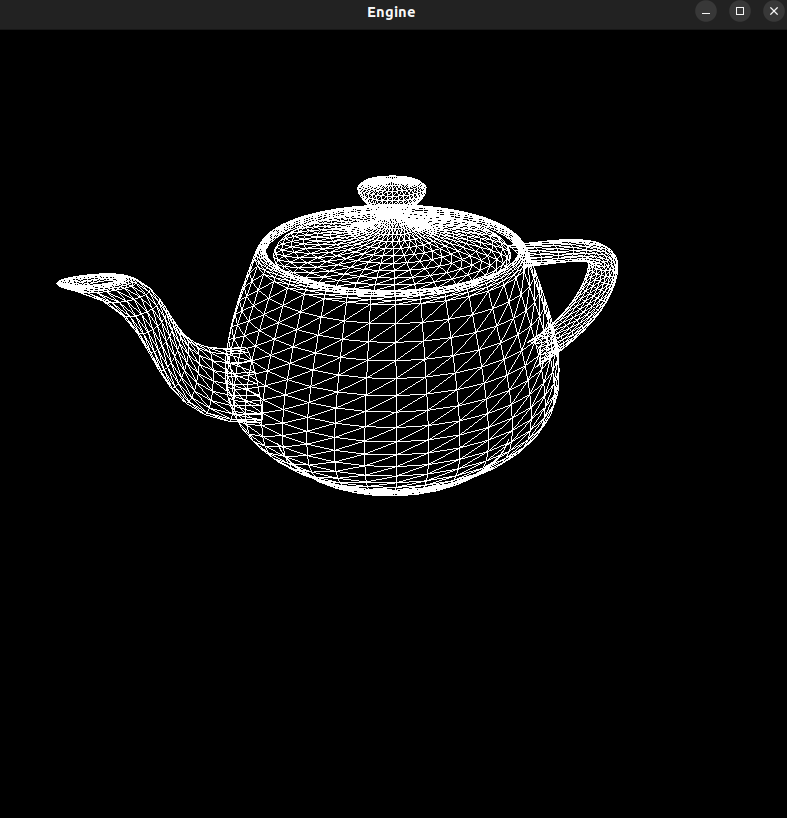
\includegraphics[width=0.8\textwidth]{imgs/teapot.png}
    \captionof{figure}{Chaleira construída com Bezier Patches}
    \label{fig:teapot}
\end{center}

\subsection{Sistema Solar num instante}

\begin{center}
    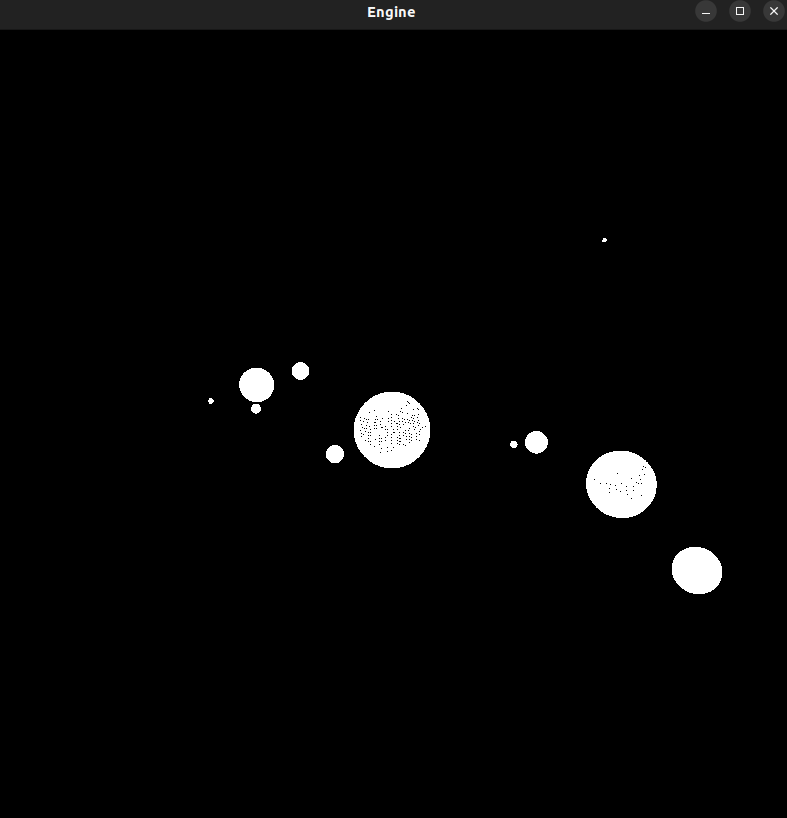
\includegraphics[width=0.8\textwidth]{imgs/sisolar1.png}
    \captionof{figure}{Sistema Solar animado num instante}
    \label{fig:sisolar1}
\end{center}

\subsection{Sistema Solar noutro instante}

\begin{center}
    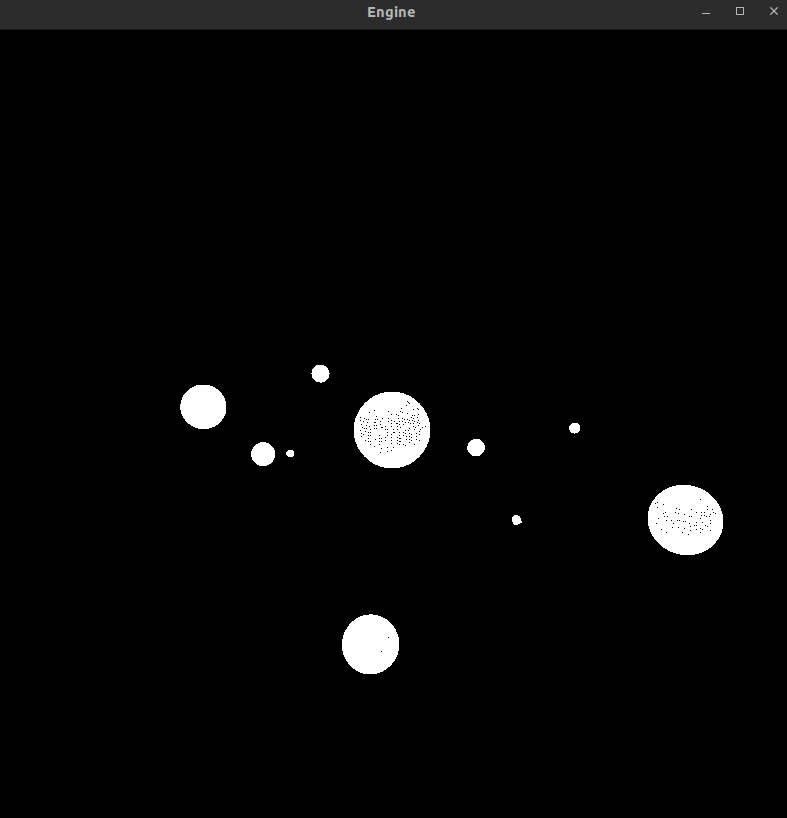
\includegraphics[width=0.8\textwidth]{imgs/sisolar2.png}
    \captionof{figure}{Sistema Solar animado noutro instante}
    \label{fig:sisolar2}
\end{center}

